\subsection{Evaluation setup}
\textbf{Agent architecture.} We evaluate agents under the ReAct~\citep{yao2023react} framework in the seven configurations of Table~\ref{tab:modes}. The \textbf{interact} action presents a yes-or-no question to the simulated user, who must respond ``yes'', ``no'', or ``I don't know''.

\textbf{Prompting strategy.} \fininteract evaluates interactive agents under several interaction protocols: answer-only, answer with search, answer with search and interaction, and the category-conditioned policies. All models run under the same ReAct system prompt. Additional details are in Appendix~\ref{sec:error}.

\textbf{Models.} We evaluate a diverse set of models. The proprietary set comprises the GPT family (GPT-5.6, GPT-5, GPT-4o, and GPT-5-mini), Claude-Sonnet-5, Gemini-3.5-flash, Grok-4.5, DeepSeek-V4-flash, GLM-5.2, and Kimi-K3. The open-source set comprises the dense Qwen3 family (4B, 8B, 14B, and 32B) and two mixture-of-experts models, Qwen3-30B-A3B and Qwen3.5-35B-A3B. Proprietary models are accessed through a unified OpenRouter harness.

\subsection{Overall performance}
\label{sec:ceiling}
Even frontier models are vulnerable to financial report ambiguity (Table~\ref{tab:main}). No model exceeds $44\%$ accuracy on the intended interpretation under free interaction, and the ceiling is low for proprietary and open-source models alike: the best full-scale model reaches $28.9\%$ and the best cross-vendor pilot model $44.0\%$.

The opportunity to interact does not by itself improve accuracy. The interaction difference $\Delta$ (added-interaction minus plain-search accuracy) is non-positive for eleven of the sixteen evaluated models, so the failure is not one of asking but of converting a clarified intention into the correct answer. For the three proprietary models we run with full interaction diagnostics this reading is direct: they interact on $96$--$99\%$ of instances and target a true ambiguity category at AC@1 $0.86$--$0.94$, so they do recognize which kind of ambiguity is present and do ask about it, yet still answer wrongly. The open models interact far less often ($15$--$72\%$), so their negative $\Delta$ mixes under-asking with the same integration failure.

Two ablations bracket this gap (Table~\ref{tab:ceiling}). Forcing four rounds of clarification \emph{lowers} accuracy rather than raising it, which is consistent with agents getting lost in multi-turn conversations~\citep{laban2026llms}. Supplying the disambiguating context $C$ as an oracle instead lifts every model to $93$--$95\%$. Because $C$ never contains the final answer $A$, this improvement shows that the gap is not missing knowledge but the ability to resolve the interpretation and carry it into the answer. Appendix~\ref{app:maindetails} reports the full analysis. \textbf{Finding 1: models can observe the ambiguity and answer correctly once the intention is made explicit, but fail to bridge the intermediate step from an updated intention to the correct answer.}

\begin{table}[t]
\centering
\caption{Forcing more clarification does not help accuracy, but \emph{resolving} the ambiguity lifts every model to $93$--$95\%$. The gap is therefore the model's inability to elicit $C$ for itself, not missing knowledge or grounding. Abbreviations follow Table~\ref{tab:modes}.}
\label{tab:ceiling}
\small
\begin{tabular}{lcccc}
\toprule
Model & A & A+I & Forced(4) & \textbf{Oracle} \\
\midrule
GPT-5      & 0.6 & 20.2 & 1.5 & \textbf{95.4} \\
GPT-4o     & 0.6 & 4.6  & 0.0 & \textbf{93.1} \\
GPT-5-mini & 0.6 & 0.0  & 0.6 & \textbf{95.4} \\
Qwen3-30B   & 1.2 & 11.6 & -- & \textbf{90.2} \\
Qwen3.5-35B & 0.6 & 28.9 & -- & \textbf{91.9} \\
\bottomrule
\end{tabular}
\end{table}

\newlength{\midgap}\setlength{\midgap}{-0.02\textwidth}% <-- gap between the two panels; adjust here
\begin{table*}[t]
\centering
\caption{\textbf{(a)}~Main results, reporting accuracy (\%) against the \emph{intended}
interpretation per mode, with $\Delta$ the +Interact minus +Search difference (full-scale rows are
$N{=}173$ and the cross-vendor frontier rows, IR and ECE blank, are a preliminary $N{=}50$ pilot).
\textbf{(b)}~Re-grading the same outputs against the intended versus the default reading a conventional benchmark would treat as gold (Same abbreviation as Table~\ref{tab:modes}). \textbf{(c)}~Per-category targeting
(AC@1), where recognition policy is a shared blind spot ($=0$ for every model). Category
sizes: entity (Ent.) 94, metric (Met.) 63, recognition (Rec.) 9, temporal (Tmp.) 7.}
\label{tab:main}
%
\begin{minipage}[t]{0.57\textwidth}
\centering
\textbf{(a) Main results}\par\smallskip
{\small\setlength{\tabcolsep}{2.5pt}
\begin{tabular}{lccccccc}
\toprule
& \multicolumn{2}{c}{Acc (\%)} &
  \multicolumn{5}{c}{Answer+Search+Interact} \\
\cmidrule(lr){2-3}\cmidrule(lr){4-8}
Model & A & A+S & A+S & $\Delta$ & IR & AC@1 & ECE \\
\midrule
\multicolumn{8}{l}{\textit{Proprietary models}} \\
GPT-5.6           & 10.0 & 36.0 & 30.0 & $-6$  & -- & .98 & -- \\
GPT-5             & 0.6 & 6.4  & \textbf{20.2} & $+13.8$ & 98.8 & .86 & .53 \\
GPT-4o            & 0.6 & 12.1 & 4.6  & $-7.5$  & 99.4 & .94 & .82 \\
GPT-5-mini        & 0.6 & 0.0  & 0.0  & $0.0$   & 96.0 & .94 & .00 \\
Claude-Sonnet-5   & 4.0  & \textbf{46.0} & \textbf{44.0} & $-2$  & -- & .98 & -- \\
Grok-4.5          & 2.0  & 40.0 & 32.0 & $-8$  & -- & .87 & -- \\
GLM-5.2           & 12.0 & 40.0 & 40.0 & $0$   & -- & .96 & -- \\
Kimi-K3           & 16.0 & 38.0 & 34.0 & $-4$  & -- & .98 & -- \\
DeepSeek-V4-flash & 12.0 & 28.0 & 24.0 & $-4$  & -- & .96 & -- \\
Gemini-3.5-flash  & 14.0 & 6.0  & 30.0 & $+24$ & -- & .96 & -- \\
\midrule
\multicolumn{8}{l}{\textit{Open source models}} \\
Qwen3-4B          & 0.0 & 8.1  & 12.1 & $+4.0$  & 28 & .85 & -- \\
Qwen3-8B          & 0.6 & 14.4 & 24.9 & $+10.5$ & 15 & .88 & -- \\
Qwen3-14B         & 0.0 & 18.5 & 22.5 & $+4.0$  & 36 & .74 & -- \\
Qwen3-32B         & 1.2 & 27.2 & 8.4  & $-18.8$ & 61 & .96 & -- \\
Qwen3-30B-A3B     & 1.2 & 28.3 & 11.6 & $-16.7$ & 72 & .90 & -- \\
Qwen3.5-35B-A3B   & 0.6 & \textbf{35.8} & 28.9 & $-6.9$ & 36 & .81 & -- \\
\midrule
\multicolumn{8}{l}{\textit{Human baseline ($N{=}50$)}} \\
Human             & -- & -- & \textbf{30.0} & -- & 100 & .72 & -- \\
\bottomrule
\end{tabular}}
\end{minipage}\hspace{\midgap}%
\begin{minipage}[t]{0.45\textwidth}
\centering
\textbf{(b) Single-gold illusion}\par\smallskip
{\small
\begin{tabular}{p{1cm}lccc}
\toprule
Model & Mode & Intended & Default & $\Delta$ \\
      &      & (true Acc) & (single-gold) & \\
\midrule
\multirow{3}{1cm}{GPT-5}  & A   & 0.6  & 2.3  & +1.7 \\
       & A+S & 6.4  & 10.4 & +4.0 \\
       & A+S+I & \textbf{20.2} & 12.1 & $-8.1$ \\
\midrule
\multirow{3}{1cm}{GPT-4o} & A & 0.6  & 0.6  & 0.0 \\
       & A+S & 12.1 & \textbf{37.0} & \textbf{+24.9} \\
       & A+S+I & 4.6  & 6.4  & +1.8 \\
\midrule
\multirow{3}{1cm}{GPT-5-mini} & A & 0.6 & 0.0 & $-0.6$ \\
           & A+S & 0.0 & 0.0 & 0.0 \\
           & A+S+I & 0.0 & 0.0 & 0.0 \\
\bottomrule
\end{tabular}}
\par\bigskip
\textbf{(c) Per-category targeting (AC@1)}\par\smallskip
{\small
\begin{tabular}{lcccc}
\toprule
Model & Ent. & Met. & Rec. & Tmp. \\
\midrule
GPT-5    & .89 & .92 & \textbf{.00} & 1.00 \\
GPT-4o   & 1.00 & .97 & \textbf{.00} & 1.00 \\
GPT-5-m  & .99 & 1.00 & \textbf{.00} & 1.00 \\
Q3-30B   & .93 & .96 & \textbf{.00} & 1.00 \\
Q3.5-35B & .85 & .87 & \textbf{.00} & 1.00 \\
\bottomrule
\end{tabular}}
\end{minipage}
\end{table*}


\subsection{Failure of existing benchmarks}
\label{sec:illusion}

Because every instance carries both a default and an intended answer, we can re-grade the \emph{identical} model outputs under the two conventions and read off what a conventional single-gold benchmark would have reported (Table~\ref{tab:main}(b)). In the retrieval-augmented regime where such benchmarks operate, grading against the default inflates the score sharply: GPT-4o is credited $37.0\%$ against the default but only $12.1\%$ against the intended reading, so a single-gold benchmark would have reported $3.1\times$ its true competence. The inflation reverses only under interaction, where GPT-5 scores $20.2\%$ intended against $12.1\%$ default, which is precisely the point: asking is what converts a default-anchored guess into the intended answer, and it is the one behavior single-gold grading cannot see. Appendix~\ref{app:maindetails} reports the full re-grading together with a human study confirming that annotators shown only $Q$ and the passage record the default reading as gold $66\%$ of the time. \textbf{Finding 2: a single-gold convention overstates competence by up to $3.1\times$, because one gold answer per question encodes the default reading rather than the intended one.}



\subsection{Targeting varies by ambiguity category}
\label{sec:skills}
Aggregate AC@1 hides where clarification actually succeeds, so we decompose targeting by ambiguity category (Table~\ref{tab:main}(c)). Models name the correct category almost always for entity scope, metric definition, and temporal scope, but never for recognition policy, where AC@1 is $0$ for every model evaluated. A case study makes the missed distinction concrete. Asked ``What were General Electric's revenues?'', a model may answer \$67.95B or \$26.79B depending on the recognition basis: the former is GAAP revenue combining over-time service recognition with point-in-time product recognition, the latter counts only revenue recognized at a point in time. Models return a single figure without asking which basis is meant, defaulting to the assumption that ``revenue'' is well defined and passing over the ASC~606 distinction between point-in-time and over-time recognition. We read this as evidence that a domain-specific reporting practice is not reflected in current models' general clarification behavior, which is what motivates the category-conditioned interventions of Sec.~\ref{sec:trainsignal}.

This last observation carries an important caveat. Recognition policy is one of our three exploratory categories, with only $n{=}9$ instances, and an item-level audit (Appendix~\ref{app:limitations}) finds most of them to be ASC~606 timing disaggregations where neither value is the total a non-expert would assume. Our two human annotators also never targeted the category, so the blind spot is at least not model-specific. We therefore report it as a preliminary observation on a small sample rather than a quantitative result, and treat entity scope ($n{=}94$) and metric definition ($n{=}63$) as the two well-powered categories. \textbf{Finding 3: targeting accuracy is uneven across ambiguity categories; entity, metric, and temporal ambiguity are reliably named, while recognition policy is never raised, on preliminary evidence from a nine-instance category.}

\subsection{Ambiguity category as training signal}
\label{sec:trainsignal}
The diagnosis so far is descriptive, so we ask whether the ambiguity category can also serve as a training signal. We run category-conditioned training on a Qwen3-4B policy, supervised fine-tuning on category-guided demonstrations followed by reinforcement learning, teaching the model to interact and to target the correct category. On the held-out split the leak-proof signals rise almost entirely at the supervised stage, with AC@1 going from $25$ to $69$ and interaction from $55$ to $100$ (Table~\ref{tab:grpo}, Figure~\ref{fig:grpo}a), while the later stages move within run-to-run noise at $n{=}51$. Full multi-turn reinforcement learning confirms that the episode is trainable end to end, with clarifying turns rising from $5.7$ to $8.6$ (Figure~\ref{fig:grpo}b). At inference time the same idea, conditioning on the category, lifts GPT-5 from $34.0\%$ to $46.0\%$ on a stratified $N{=}50$ pilot (Appendix~\ref{sec:axisreact}). The gains concentrate on the data-abundant categories, so the signal is actionable but does not reach the recognition-policy blind spot of Sec.~\ref{sec:skills}. Additional details are in Appendix~\ref{sec:grpo}. \textbf{Finding 4: conditioning on the ambiguity category improves clarification at both training and inference time, so \fininteract provides an actionable signal and not only a diagnosis.}

\begin{table}[t]
\centering
\caption{RLVR ladder on \fininteract with Qwen3-4B, held-out $n{=}51$. Category-guided supervision installs on-category clarification, with the leak-proof signals (AC@1 and interaction) rising almost entirely at the SFT stage. Accuracy is leak-confounded and is reported for completeness only.}
\label{tab:grpo}
\small
\begin{tabular}{lcccc}
\toprule
Stage & AC@1 & Interaction & Accuracy & Reward \\
\midrule
Base      & 25.0 & 54.9 & 84.3 & 0.96 \\
\;\;+\,SFT & 68.6 & \textbf{100} & 88.2 & 1.28 \\
\;\;+\,KTO               & \textbf{70.6} & \textbf{100} & 84.3 & 1.27 \\
\;\;+\,GRPO              & 66.7 & \textbf{100} & 88.2 & \textbf{1.30} \\
\bottomrule
\end{tabular}
\end{table}

\begin{figure*}[t]
\centering
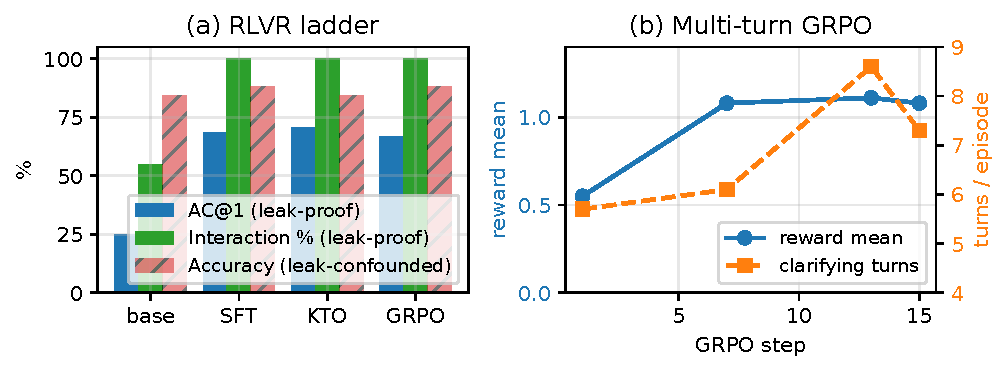
\includegraphics[width=0.9\textwidth]{fig_grpo_insights.pdf}
\caption{\textbf{Category-guided training installs on-category clarification.} (a) The leak-proof signals, AC@1 and interaction rate, jump at the supervised stage and change little thereafter. (b) True multi-turn GRPO on the 4B policy: mean reward and clarifying turns rise together over training.}
\label{fig:grpo}
\end{figure*}